\subsection{Zernike modes PSFs Clustering}

	\subsubsection{UMAPS}
		
		Before clustering, UMAPS for flattened PSF matrices, flattend LP coefficients matrices and PL intensities are processed. The same configuration is used for the different number of modes.
		
		\begin{table}[h!]
			\centering
			\begin{tabular}{|c|c|c|c|}
				\hline
				\textbf{Dataset type} & \textbf{Number of neighbors} & \textbf{Min distance} & \textbf{Number of components} \\
				\hline
				Zernike modes PSF & 500 & 0.3 & 3 \\
				\hline
				LP coefficients & 500 & 0.1 & 2 \\
				\hline
				PL intensities & 500 & 0.1 & 2 \\
				
				\hline
			\end{tabular}
		\caption{UMAP parameter configurations for each of the dataset type}
		\end{table}
		
		The resulting projections are the following:
		\begin{figure*}[ht!]
			\centering
			\subfloat[2 Zernike modes LP coefficients UMAP]{%
			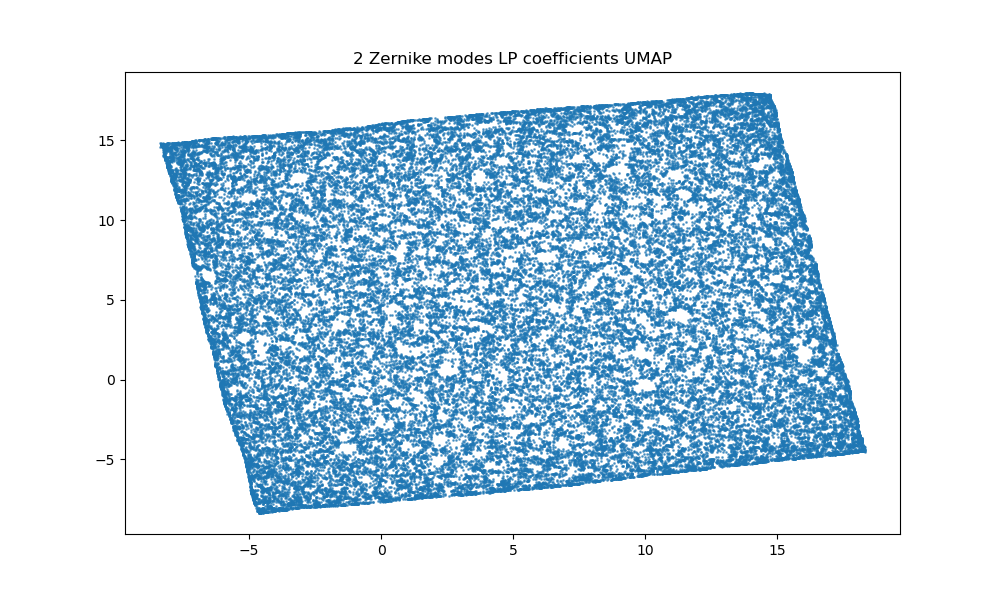
\includegraphics[ width=0.31\textwidth]{pid-2mlpumap.png}}
			\hspace{\fill}
			\subfloat[2 Zernike modes PL intensities UMAP]{%
			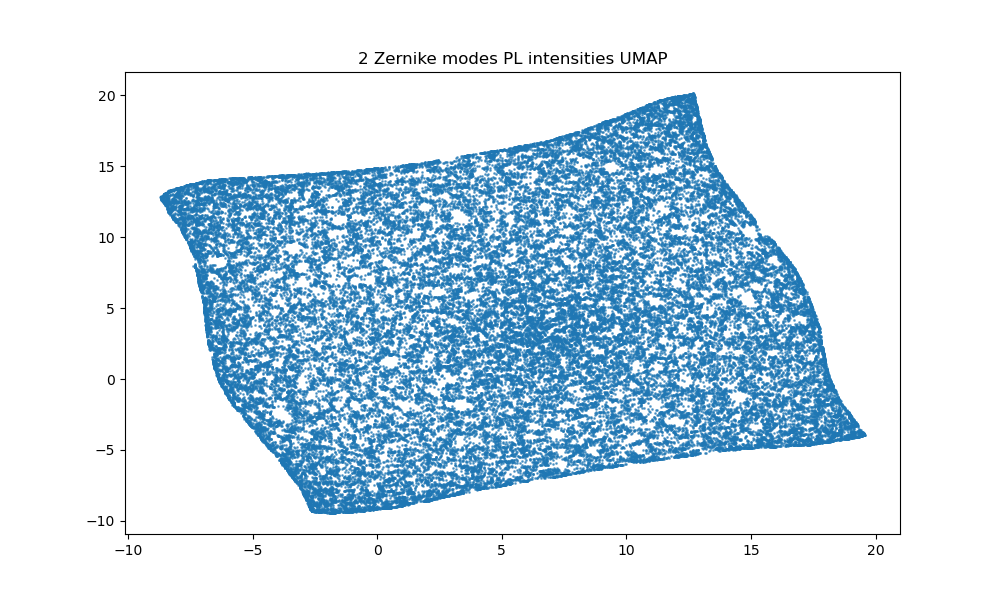
\includegraphics[ width=0.31\textwidth]{pid-2mplumap.png}}
			\hspace{\fill}
			\subfloat[2 Zernike modes PSF UMAP]{%
			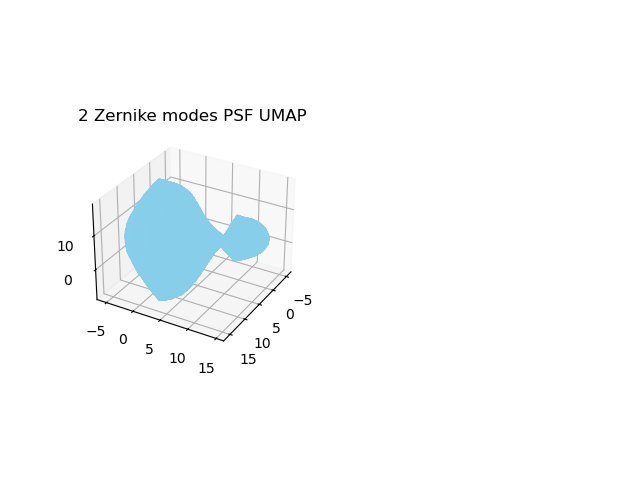
\includegraphics[ width=0.31\textwidth]{pid-2mpsfumap.png}}
			\\
			
			\subfloat[5 Zernike modes LP coefficients UMAP]{%
			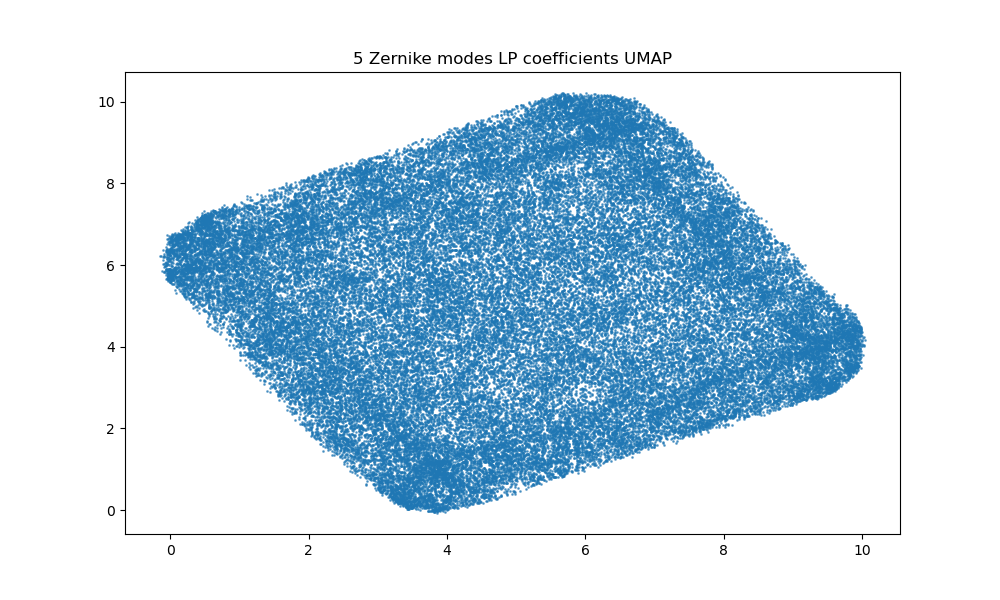
\includegraphics[ width=0.31\textwidth]{pid-5mlpumap.png}}
			\hspace{\fill}
			\subfloat[5 Zernike modes PL intensities UMAP]{%
			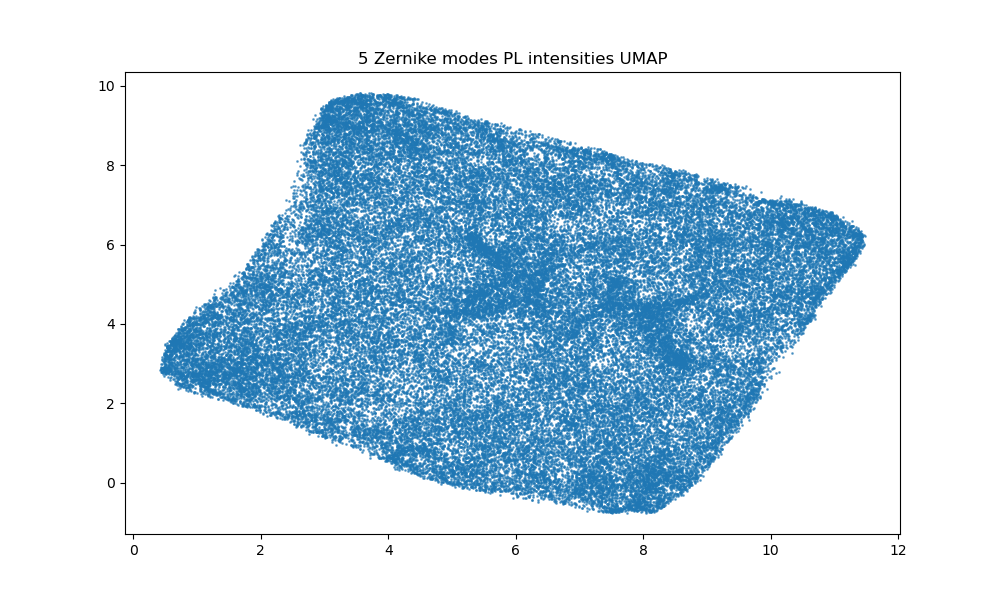
\includegraphics[ width=0.31\textwidth]{pid-5mplumap.png}}
			\hspace{\fill}
			\subfloat[5 Zernike modes PSF UMAP]{%
			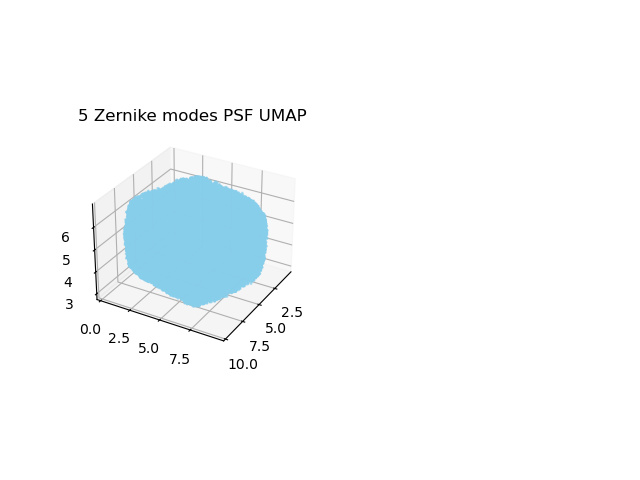
\includegraphics[ width=0.31\textwidth]{pid-5mpsfumap.png}}
			\\
			
			\subfloat[9 Zernike modes LP coefficients UMAP]{%
			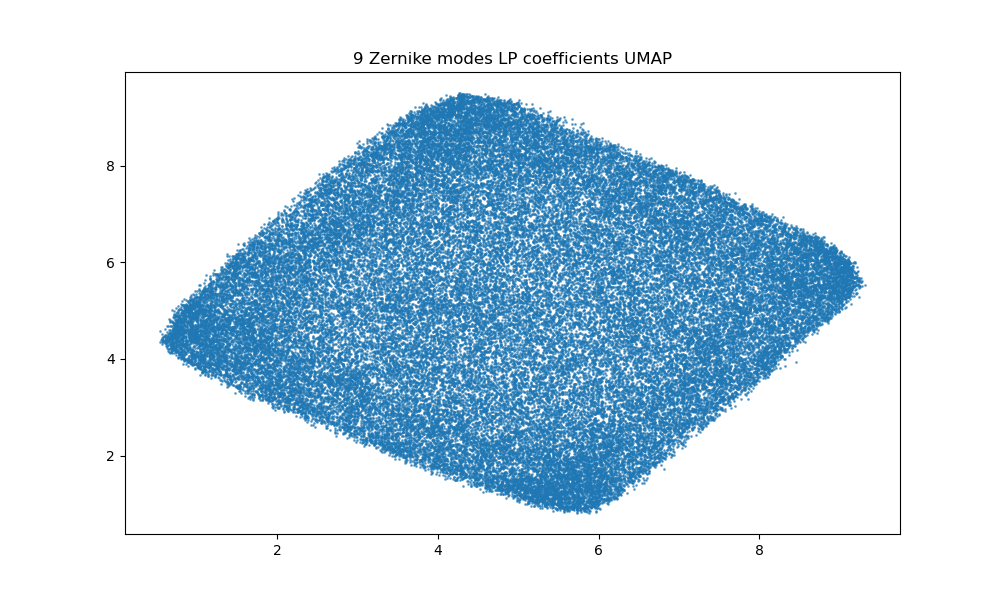
\includegraphics[ width=0.31\textwidth]{pid-9mlpumap.png}}
			\hspace{\fill}
			\subfloat[9 Zernike modes PL intensities UMAP]{%
			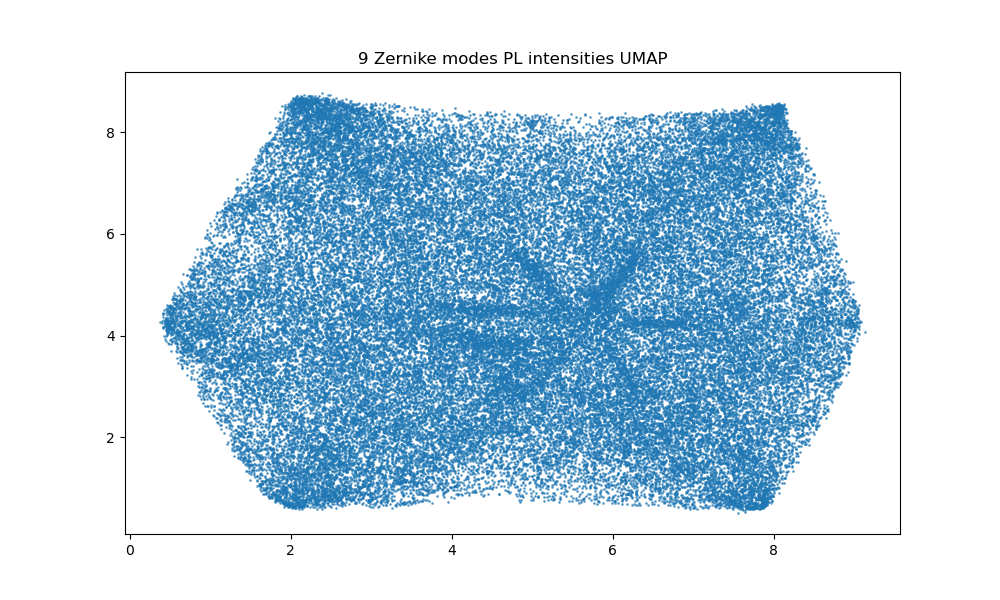
\includegraphics[ width=0.31\textwidth]{pid-9mplumap.png}}
			\hspace{\fill}
			\subfloat[9 Zernike modes PSF UMAP]{%
			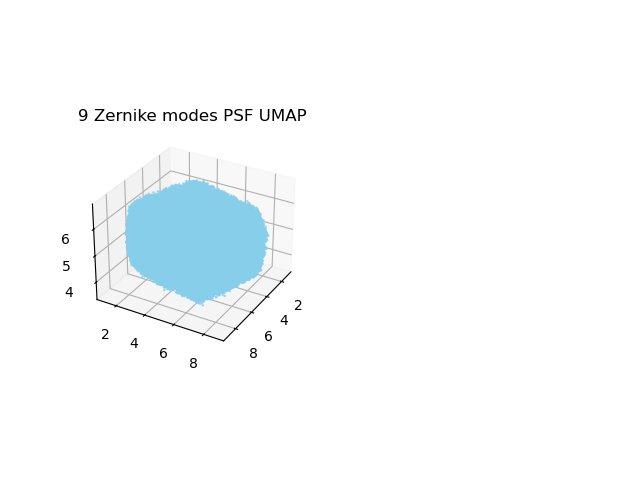
\includegraphics[ width=0.31\textwidth]{pid-9mpsfumap.png}}
			\\
			
			\subfloat[14 Zernike modes LP coefficients UMAP]{%
			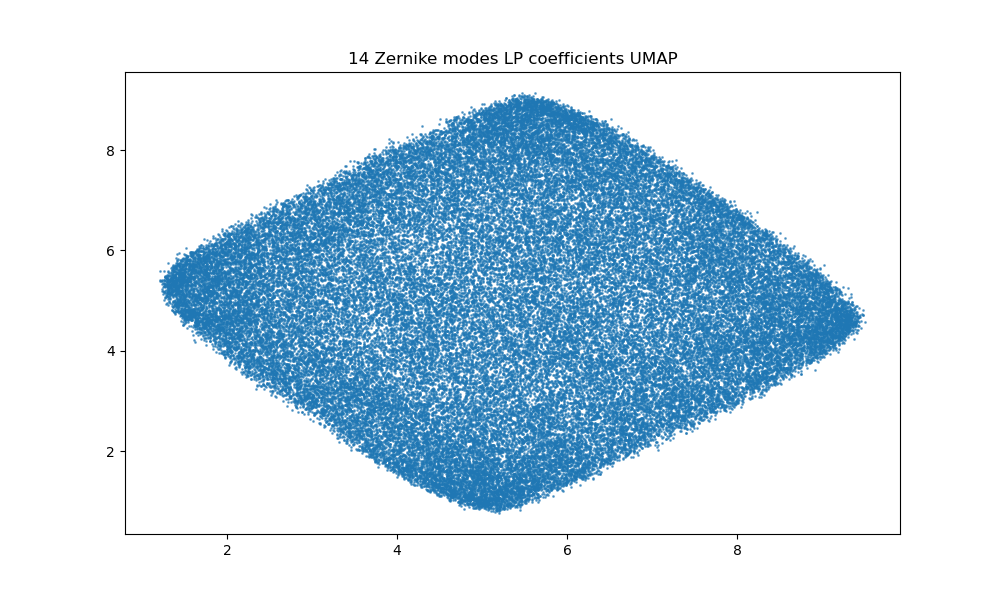
\includegraphics[ width=0.31\textwidth]{pid-14mlpumap.png}}
			\hspace{\fill}
			\subfloat[14 Zernike modes PL intensities UMAP]{%
			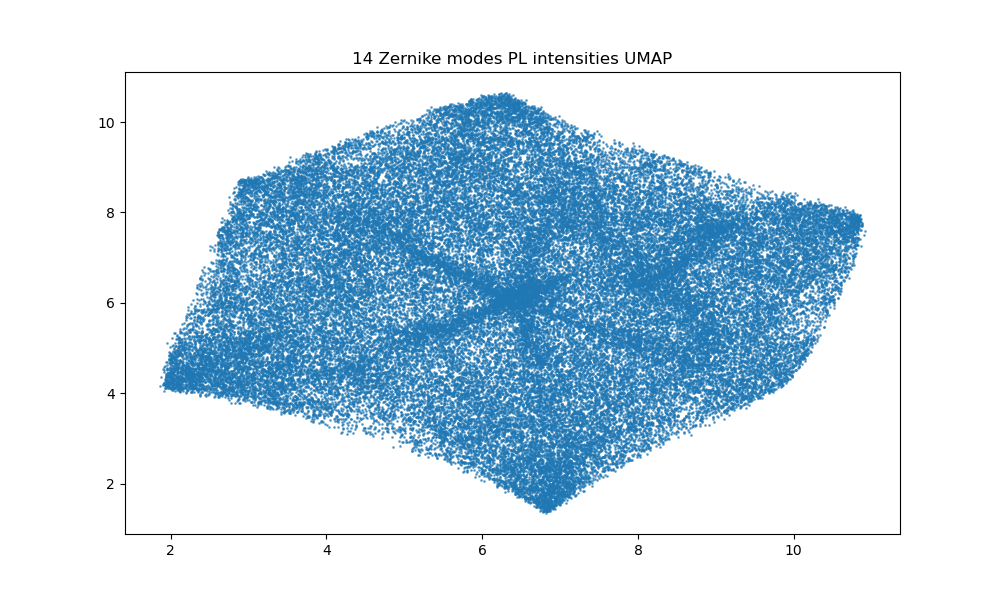
\includegraphics[ width=0.31\textwidth]{pid-14mplumap.png}}
			\hspace{\fill}
			\subfloat[14 Zernike modes PSF UMAP]{%
			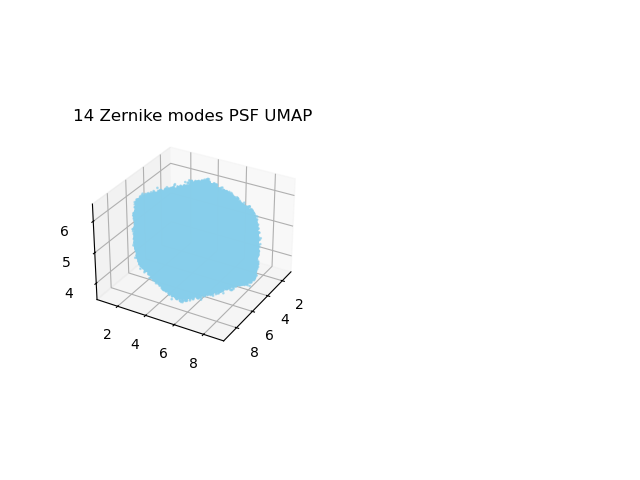
\includegraphics[ width=0.31\textwidth]{pid-14mpsfumap.png}}
			\\
			
			\subfloat[20 Zernike modes LP coefficients UMAP]{%
			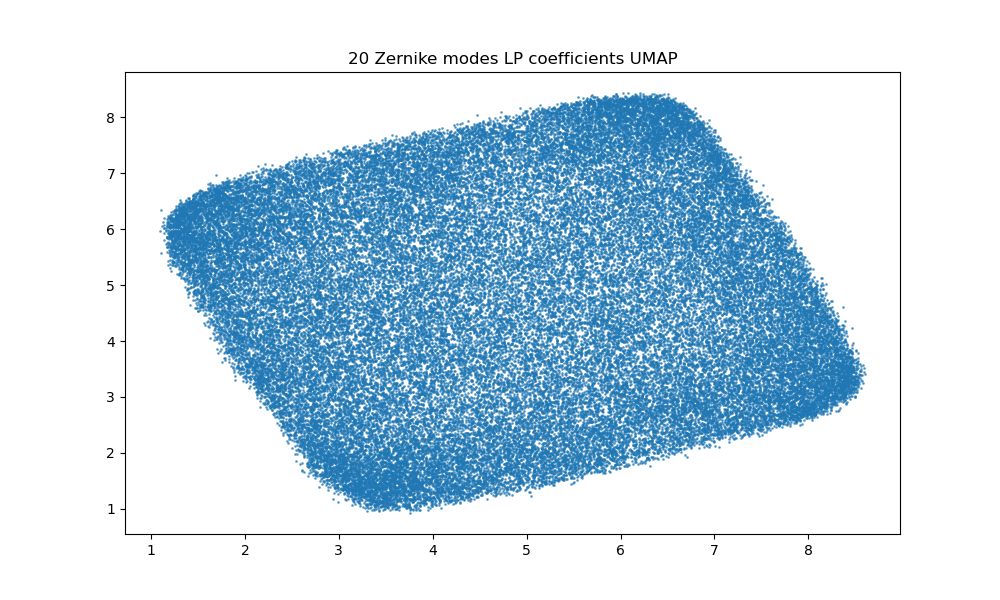
\includegraphics[ width=0.31\textwidth]{pid-20mlpumap.png}}
			\hspace{\fill}
			\subfloat[20 Zernike modes PL intensities UMAP]{%
			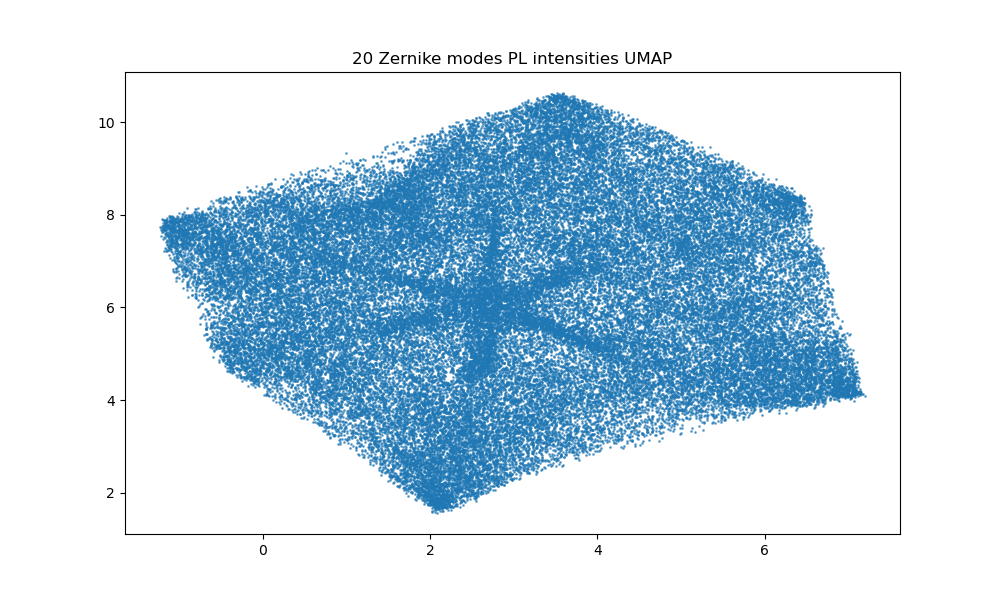
\includegraphics[ width=0.31\textwidth]{pid-20mplumap.png}}
			\hspace{\fill}
			\subfloat[20 Zernike modes PSF UMAP]{%
			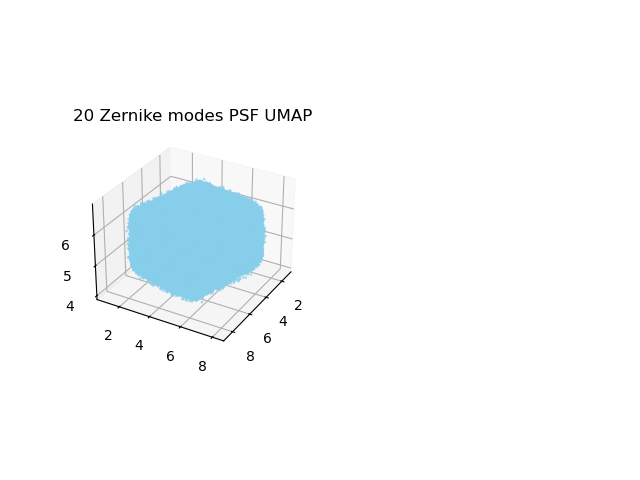
\includegraphics[ width=0.31\textwidth]{pid-20mpsfumap.png}}
			\\
			
			\caption{Datasets UMAPs}
		\end{figure*}
		\FloatBarrier
		
	
	\subsubsection{Clustering}
		
		Using DBSCAN, clusters are defined in each dataset.
		
		\paragraph{2 Zernike modes}:
		\begin{table}[h!]
			\centering
			\begin{tabular}{|c|c|c|c|c|}
				\hline
				\textbf{} & \textbf{PSF} & \textbf{LP coeffs} & \textbf{PL intensities} & \textbf{Pred PSF}\\
				\hline
				\textbf{DBSCAN $\epsilon$} &  & 0.11 & 0.102 0.102 & \\
				\hline
				\textbf{DBSCAN neighbors} &  & 6 & 4 & \\
				\hline
				\textbf{Number of clusters} &  & 1447 & 1553 & \\
				\hline
				\textbf{Cluster density mean} &  & 42.37 & 41.59 & \\
				\hline
				\textbf{Cluster density variance} &  & 157.86 & 64594 & \\
				\hline
				\textbf{Non noise points} &  & 61313 & \\
				\hline
			\end{tabular}
		\caption{Clustering for 2 Zernike modes datasets}
		\end{table}
		
		\paragraph{5 Zernike modes}:
		\begin{table}[h!]
			\centering
			\begin{tabular}{|c|c|c|c|c|}
				\hline
				\textbf{} & \textbf{PSF} & \textbf{LP coeffs} & \textbf{PL intensities} & \textbf{Pred PSF}\\
				\hline
				\textbf{DBSCAN $\epsilon$} &  & 0.0385 & 0.041 & \\
				\hline
				\textbf{DBSCAN neighbors} &  & 5 & 5 & \\
				\hline
				\textbf{Number of clusters} &  & 1601 & 1527 & \\
				\hline
				\textbf{Cluster density mean} &  & 39.42 & 41.43 & \\
				\hline
				\textbf{Cluster density variance} &  & 348.27 & 273.60 & \\
				\hline
				\textbf{Non noise points} &  & 63120 & 63266 & \\
				\hline
			\end{tabular}
		\caption{Clustering for 5 Zernike modes datasets}
		\end{table}
		
		\paragraph{9 Zernike modes}:
		\begin{table}[h!]
			\centering
			\begin{tabular}{|c|c|c|c|}
				\hline
				\textbf{} & \textbf{PSF} & \textbf{LP coeffs} & \textbf{PL intensities}\\
				\hline
				\textbf{DBSCAN $\epsilon$} &  & 0.0335 & \\
				\hline
				\textbf{DBSCAN neighbors} &  & 6 & \\
				\hline
				\textbf{Number of clusters} &  & 1649 & \\
				\hline
				\textbf{Cluster density mean} &  & 37.05 & \\
				\hline
				\textbf{Cluster density variance} &  & 239.01 & \\
				\hline
				\textbf{Non noise points} &  & 61106 & \\
				\hline
			\end{tabular}
		\caption{Clustering for 9 Zernike modes datasets}
		\end{table}
		
		\paragraph{14 Zernike modes}:
		\begin{table}[h!]
			\centering
			\begin{tabular}{|c|c|c|c|}
				\hline
				\textbf{} & \textbf{PSF} & \textbf{LP coeffs} & \textbf{PL intensities}\\
				\hline
				\textbf{DBSCAN $\epsilon$} &  & 0.0322 & \\
				\hline
				\textbf{DBSCAN neighbors} &  & 6 & \\
				\hline
				\textbf{Number of clusters} &  & 1472 & \\
				\hline
				\textbf{Cluster density mean} &  & 41.82 & \\
				\hline
				\textbf{Cluster density variance} &  & 330.54 & \\
				\hline
				\textbf{Non noise points} &  & 61570 & \\
				\hline
			\end{tabular}
		\caption{Clustering for 14 Zernike modes datasets}
		\end{table}
		
		\paragraph{20 Zernike modes}:
		\begin{table}[h!]
			\centering
			\begin{tabular}{|c|c|c|c|}
				\hline
				\textbf{} & \textbf{PSF} & \textbf{LP coeffs} & \textbf{PL intensities}\\
				\hline
				\textbf{DBSCAN $\epsilon$} &  & 0.031 & \\
				\hline
				\textbf{DBSCAN neighbors} &  & 6 & \\
				\hline
				\textbf{Number of clusters} &  & 1596 & \\
				\hline
				\textbf{Cluster density mean} &  & 38.09 & \\
				\hline
				\textbf{Cluster density variance} &  & 305.13 & \\
				\hline
				\textbf{Non noise points} &  & 60804 & \\
				\hline
			\end{tabular}
		\caption{Clustering for 20 Zernike modes datasets}
		\end{table}